\subsection{\textit{SARTRE}}\label{sec:SARTRE}

% /include SARTRE notes from Michal/
% \par
\acrshort{sartre} \cite{Chan2012ProjectSARTRE} stands for Safe Road Trains for the Environment and it is a project which is financed by the European Union. The project is already finished, it lasted for 36 months since September 2009. Its goal was to develop a prototype of system that would be able to coordinate road-trains, so called platoons, in a way that only the first car in a platoon must be driven by a driver and all others are just following it without a need of a driver to pay attention on road. Very important for this project was the use of available technologies meaning that the system may be (in theory) implemented straight after finishing the study. Also, it was designed to work on the actual roads without the need of changing the infrastructure.\par
% 
There have been reasons for realisation of such a project. The traffic on roads is heavier every year \cite{Tencer2011NumberWheels}, meaning that there are more and more cars being driven which raises several problems: pollution, safety, traffic congestion and limited space for increasing the road capacity. These were the main reasons for realisation of \acrshort{sartre}. \par
% 
As already mentioned, the main goal was to develop system that would be able to handle platooning. The idea is that in the first vehicle (so called lead vehicle - LV) would be a trained driver which is followed by other vehicles (following vehicles - FV) that after joining a platoon become fully autonomous. Therefore, there are three categories of vehicles with which the system would interact: lead, following and other non-platooning vehicles. The reason is that platoons would be driving down the normal highways mixed with normal (non-platooning) traffic. The system must be able to handle this as there may many cases of direct interaction of the platoon with other vehicles (a vehicle interrupting the platoon by breaking in between two cars, etc.). This however, has not been covered deeply by this project, they are just aware that different situations of interaction may occur and that they must be handled.\par
% 
The architecture of the system was not described to details, there has just been diagrams showing how it looked like (Figure \ref{fig:HW_FW}, showing the hardware configuration of the following vehicle, and Figure \ref{fig:HW_LW}, the configuration of leading vehicle). Also, it was not mentioned what kind (brand, model) of hardware has been used.\par
% 
\begin{figure}[t]
    \centering
    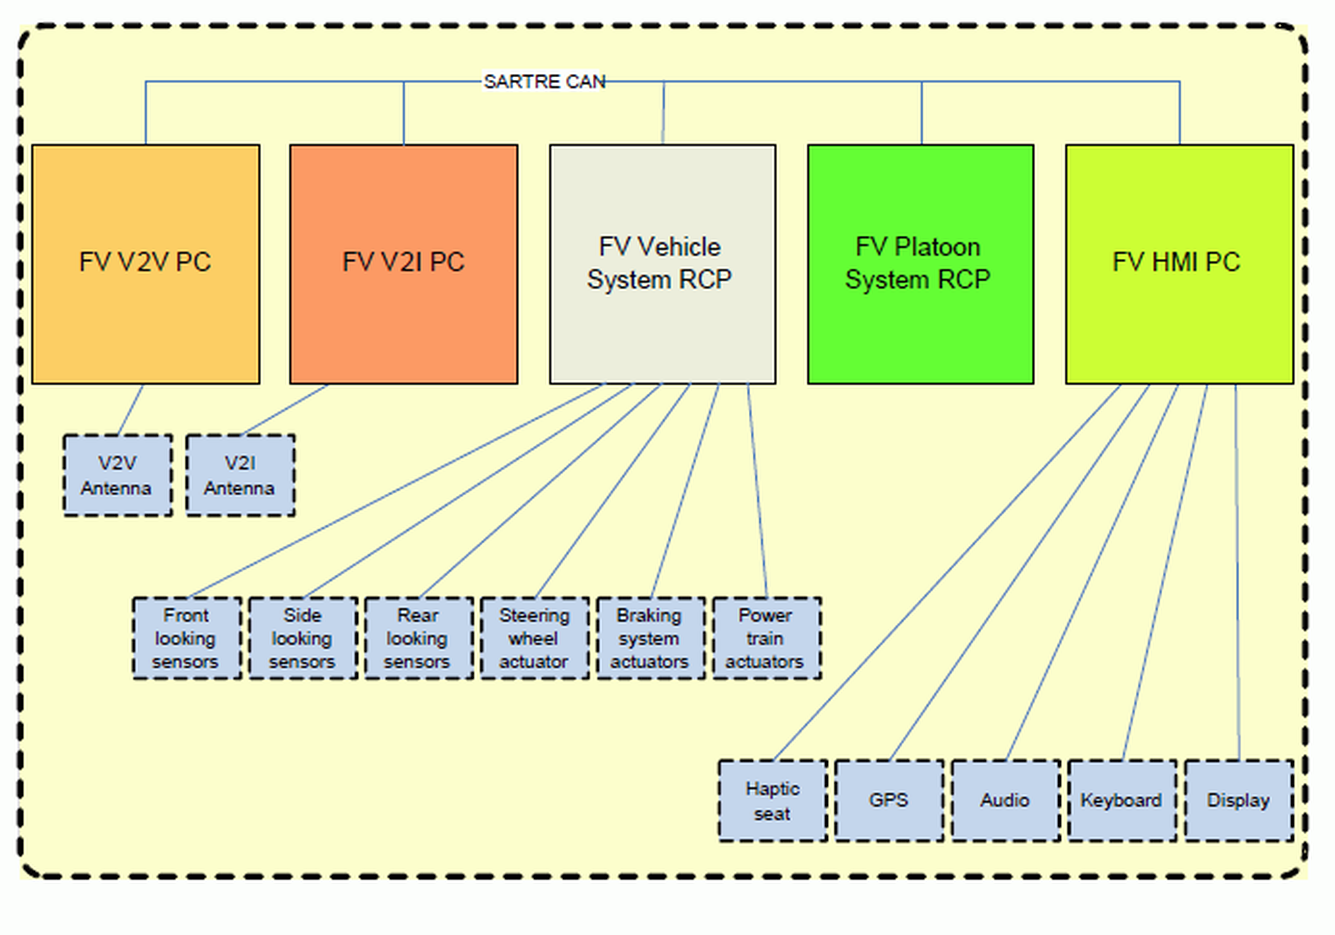
\includegraphics[width=.95\textwidth]{HW_FW}
    \caption{Hardware architecture of following vehicle (vehicle that is platooning). Taken from \cite{Chan2012ProjectSARTRE}.}
    \label{fig:HW_FW}
\end{figure}
% 
\begin{figure}[t]
    \centering
    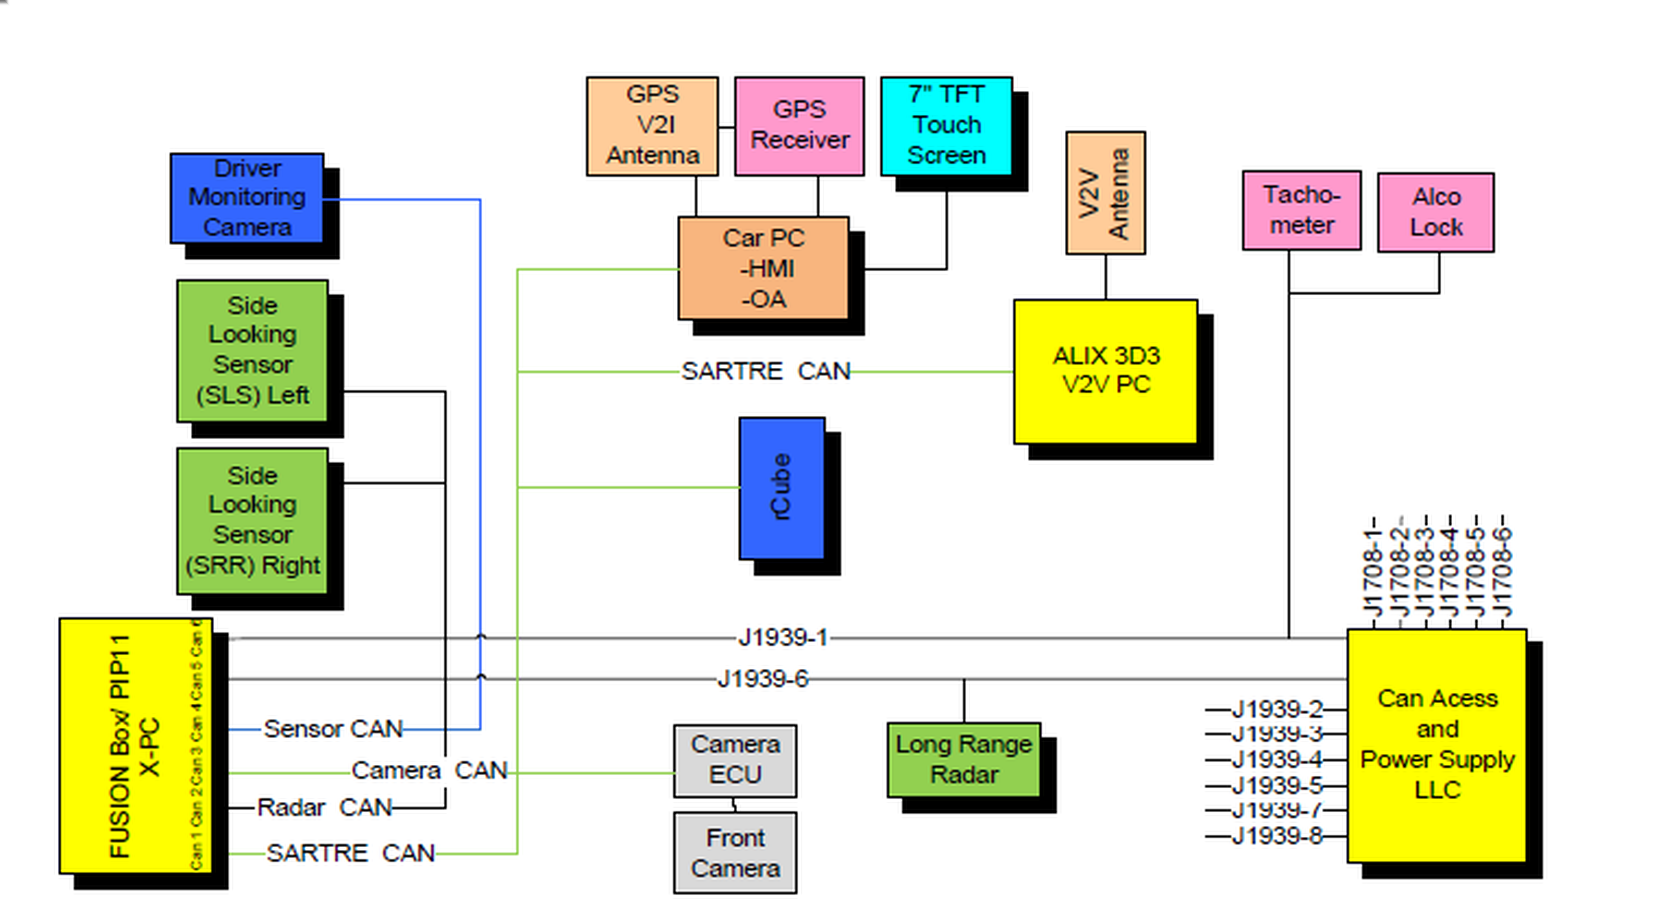
\includegraphics[width=.95\textwidth]{layoutHW}
    \caption{Hardware architecture of the leading vehicle. Taken from \cite{Chan2012ProjectSARTRE}.}
    \label{fig:HW_LW}
\end{figure}
% 
At the end the testing was conducted with truck as the leading vehicle and another truck and three cars as following vehicle. It successfully shown that it is possible to create a platoon of several vehicles where the following vehicles were driven autonomously. Also, that the fuel consumption is being reduced by approximately 10\%.